\documentclass{standalone}
\usepackage{pgfplots}
\usepgfplotslibrary{groupplots}

\begin{document}

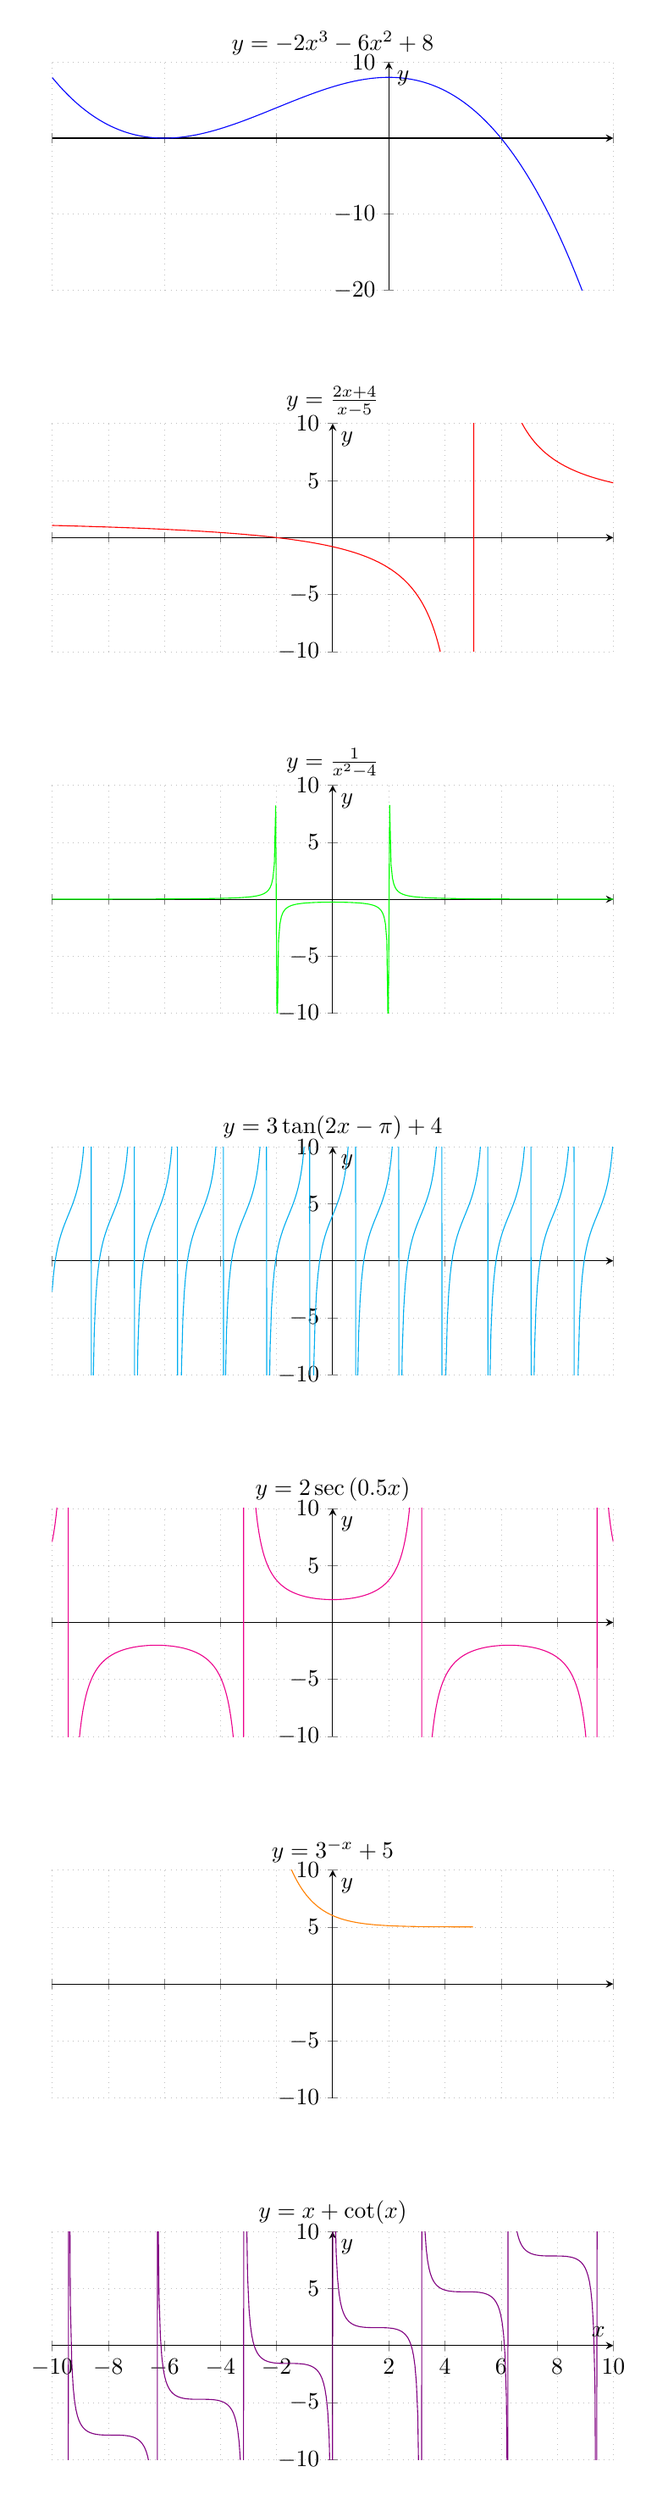
\begin{tikzpicture}
    \begin{groupplot}[
        group style={
            group size=1 by 7,
            vertical sep=2cm,
            xlabels at=edge bottom,
            ylabels at=edge left,
            xticklabels at=edge bottom,
            yticklabels at=edge left
        },
        width=10cm,
        height=5cm,
        grid=major,
        grid style={line width=.1pt, draw=gray!50, dotted},
        major grid style={line width=.2pt, draw=gray!50, dotted},
        axis lines=middle,
        xlabel={$x$},
        ylabel={$y$},
        title style={yshift=-1.5ex}, % Adjust title position
        % Customize individual plots if necessary
        title={$y = -2x^3 - 6x^2 + 8$}
    ]

    % Graph 1: y = -2x^3 - 6x^2 + 8
    \nextgroupplot[
        xmin=-3,xmax=2,
        ymin=-20,ymax=10,
        ]
    \addplot[blue, domain=-3:2, samples=400] {-2*x^3 - 6*x^2 + 8};

    % Graph 2: y = (2x + 4) / (x - 5)
    \nextgroupplot[
        xmin=-10,xmax=10,
        ymin=-10,ymax=10,
        title={$y = \frac{2x + 4}{x - 5}$}
    ]
    \addplot[red, domain=-10:10, samples=400] {(2*x + 4)/(x - 5)};

    % Graph 3: y = 1 / (x^2 - 4)
    \nextgroupplot[
        xmin=-10,xmax=10,
        ymin=-10,ymax=10,
        title={$y = \frac{1}{x^2 - 4}$}
    ]
    \addplot[green, domain=-10:10, samples=400] {1/(x^2 - 4)};

    % Graph 4: y = 3*tan(2x - pi) + 4
    \nextgroupplot[
        xmin=-10,xmax=10,
        ymin=-10,ymax=10,
        title={$y = 3\tan(2x - \pi) + 4$}
    ]
    \addplot[cyan, domain=-10:10, samples=400] {3*tan(deg(2*x - pi)) + 4};

    % Graph 5: y = 2*sec(0.5x)
    \nextgroupplot[
        xmin=-10,xmax=10,
        ymin=-10,ymax=10,
        title={$y=2\sec\left(0.5x\right)$}
    ]
    \addplot[magenta, domain=-10:10, samples=400] {2/(cos(deg(0.5*x)))};

    % Graph 6: y = 3^(-x) + 5
    \nextgroupplot[
        xmin=-10,xmax=10,
        ymin=-10,ymax=10,
        title={$y = 3^{-x} + 5$}
    ]
    \addplot[orange, domain=-5:5, samples=400] {3^(-x) + 5};

    % Graph 7: y = x + cot(x)
    \nextgroupplot[
        xmin=-10,xmax=10,
        ymin=-10,ymax=10,
        title={$y = x + \cot(x)$}
    ]
    \addplot[violet, domain=-10:10, samples=400] {x + cot(deg(x))};

    \end{groupplot}
\end{tikzpicture}




\end{document}
